% !TeX root = ../libro.tex
% !TeX encoding = utf8

\chapter{Ciencia de datos}\label{ch:octavo-capitulo}
\section{Introducción}
La ciencia de datos es un campo interdisciplinario que utiliza algoritmos, procedimientos y procesos para examinar grandes cantidades de datos con el fin de descubrir patrones ocultos, generar conocimientos y dirigir la toma de decisiones. Utiliza técnicas y teorías extraídas de muchos campos dentro del contexto de las matemáticas, estadísticas, programación, análisis, IA y aprendizaje automático para descubrir conocimientos accionables a partir de conjuntos de datos.\par

En el contexto de la astrofísica, la ciencia de datos juega un papel crucial. Los astrofísicos y físicos de partículas utilizan instrumentación de última generación en telescopios y aceleradores para estudiar el Universo tanto en las escalas más grandes como en las más pequeñas. Los enormes conjuntos de datos a escala de petabytes que resultan de las diferentes observaciones y experimentos se explotan en busca de indicios, pistas que pueden arrojar luz sobre la naturaleza de la materia oscura, la energía oscura, la evolución de los agujeros negros y la física más allá del "modelo estándar" de la cosmología y la física de partículas.\par

El desafío es reformular el modelado de datos que los astrofísicos necesitan hacer de tal manera que se puedan aplicar arquitecturas de aprendizaje automático de última generación, sin comprometer el alto nivel de control de errores sistemáticos, ni la comprensión detallada de la incertidumbre estadística, que las preguntas de física que se están abordando con extrema precisión en el siglo XXI exigen. Por lo tanto, las simulaciones nos permiten probar qué teorías son consistentes con el Universo que podemos observar. Esta es una clara demostración del poder y la necesidad de la ciencia de datos para avanzar en nuestra comprensión del universo.\par


\section{Proceso de la ciencia de datos}
El proceso de ciencia de datos es un enfoque sistemático que implica varios pasos para extraer valiosos conocimientos de los datos. Comienza con la definición del problema, que implica entender los objetivos que se persiguen y formular preguntas que pueden ser respondidas con datos. Los siguientes pasos implican la recopilación y limpieza de los datos, seguidos por el análisis exploratorio de los mismos para entender los patrones y tendencias subyacentes. Esto es continuado por la construcción y evaluación del modelo para predecir resultados o descubrir estructuras dentro de los datos. Finalmente, el modelo se despliega, se contrastan los resultados con las observaciones, y los hallazgos se comunican a las partes interesadas.\par

Desde una perspectiva científica, el proceso de ciencia de datos es crucial ya que proporciona una metodología estructurada para manejar y analizar grandes volúmenes de datos. Permite a los científicos probar hipótesis, descubrir patrones, hacer predicciones e impulsar la toma de decisiones. Cada paso en el proceso sirve a un propósito específico y contribuye al objetivo general de extraer información significativa de los datos. Por ejemplo, la limpieza de datos asegura la calidad de los datos, el análisis exploratorio de datos ayuda a entender los datos, y la construcción del modelo permite hacer predicciones e inferencias.\par

Además, la naturaleza iterativa del proceso de ciencia de datos se alinea con el método científico de investigación, que implica formar hipótesis, realizar experimentos y refinar teorías basadas en los resultados. Este proceso iterativo nos permite un aprendizaje y mejora continua. Además, el énfasis en la comunicación en el proceso de ciencia de datos asegura que los hallazgos puedan ser compartidos e implementados de manera efectiva, contribuyendo al avance del conocimiento en varios campos. Por lo tanto, el proceso de ciencia de datos no sólo es un aspecto fundamental de la toma de decisiones basada en datos, sino también un contribuyente significativo al progreso científico.\par

Dentro del proceso de datos podemos enumerar una serie de etapas encaminadas a establecer una sistemática a la hora de su ejecución. El proceso no debe contemplarse como un marco rígido que no admite alteraciones al mismos, sino como que debe ser utilizado como una herramienta que debe ser adaptada a nuestras necesidades. Dependiendo de los objetivos establecidos, de la calidad de los datos que están a nuestra disposición, algunas de las siguientes etapas se harán más necesarias que otras, más intensas en lo que a la asignación de recursos se refiere. Entre los diferentes podemos enumerar los siguientes:
 
\begin{enumerate}
	\item \textit{Definición del problema} - Este es el primer paso donde definimos el problema que estás tratando de resolver. Implica entender los objetivos de la investigación, para a continuación formular preguntas que pueden ser respondidas con datos e identificar las fuentes de datos necesarias.
	\item \textit{Recopilación de datos} - En este paso, recopilamos los datos necesarios para nuestro análisis. Esto podría implicar la consulta de sitios web, el acceso a bases de datos, generación de simulaciones.
	\item \textit{Limpieza de datos} - Una vez que tenemos los datos recopilados, es hora de limpiarlos. Esto implica manejar valores faltantes, eliminar duplicados, corregir errores y lidiar con valores atípicos.
	\item \textit{Análisis exploratorio de datos} - Este es un paso crucial donde exploramos y visualizamos los datos para entender los patrones subyacentes, las tendencias y los valores atípicos. Es una paso fundamental porque nos ayuda a generar conocimiento y formar hipótesis para un análisis más profundo.
	\item \textit{Ingeniería de características} - Esto implica crear nuevas características a partir de las existentes para representar mejor los patrones subyacentes en los datos. Es un paso esencial para mejorar el rendimiento de los modelos de aprendizaje automático. 
	\item \textit{Construcción del modelo} - Aquí, elegimos un modelo apropiado, lo entrenamos con los datos que previamente hemos obtenido para luego evaluar su rendimiento. Normalmente esto implica dividir los datos en conjuntos de entrenamiento y prueba, seleccionar un algoritmo correcto y fijar sus parámetros.
	\item \textit{Evaluación del modelo} - En este paso, evaluamos el rendimiento del utilizando métricas apropiadas. Es importante usar una métrica que se alinee con los objetivos que hemos prefijados en el paso inicial.
	\item \textit{Despliegue del modelo} - Una vez que estamos satisfecho con el rendimiento del modelo, es hora de desplegarlo. Esto podría implicar integrar el modelo en un sistema de producción, establecer un sistema de monitoreo y desarrollar un plan para el mantenimiento del mismo.
	\item \textit{Comunicación} - Finalmente, comunicamos nuestros hallazgos a las partes interesadas. Esto podría implicar la creación de artículos científicos, informes, o presentaciones que expliquen claramente tu metodología, hallazgos e implicaciones de negocio de nuestro trabajo.
\end{enumerate}

Como hemos adelantado, los pasos anteriores no de dejan de ser un marco de trabajo genérico que debe de ser adaptado a nuestras necesidades específicas. En nuestro caso en particular, no hemos recurrido al uso de herramientas de aprendizaje automático, por lo que la correspondiente etapa no ha formado parte de nuestro proceso de ciencia de datos. Del mismo modo, nuestro modelo no ha sido incorporado, integrado con ningún sistema. De momento este no ha sido el caso pero no sería una insensatez pensar que pudiese pasar a incorporarse como una extensión a la herramienta que hemos utilizado para nuestras simulaciones, si lo autores de la misma lo considerasen oportuno.

\section{Herramientas}
\subsection{Modules for Experiments in Stellar Astrophysics - (MESA)}
Para la realización de este tesis doctoral nos hemos apoyado en la herramienta de evolución estelar \textit{Modules for Experiments in Stellar Astrophysics} (MESA). MESA ha jugado un papel fundamental en nuestra investigación y por ello, debido a su importancia, le hemos dedicado un capítulo en exclusiva en el que entramos a fondo en sus características, estructura, módulos que lo componen, y muy especialmente en cómo extender la física que incorpora sus modelos mediante la programación de nuestras propias rutinas.\par


\subsection{Octave} \label{sec:tool_octave}
GNU Octave es un lenguaje de programación de alto nivel destinado principalmente a cálculos numéricos. Es un conjunto de software libre y de código abierto que proporciona una interfaz de línea de comandos conveniente para resolver problemas lineales y no lineales numéricamente. La sintaxis de Octave es en gran medida compatible con MATLAB, lo que lo convierte en una alternativa popular para los usuarios que necesitan una solución rentable. 

Octave proporciona capacidades para la solución numérica de problemas lineales y no lineales, y para realizar otros experimentos numéricos. También proporciona amplias capacidades gráficas para la visualización y manipulación de datos. Octave puede ser extendido por paquetes, permitiendo a los usuarios añadir más funcionalidades según sea necesario. Puede ser ejecutado en modo GUI, como una consola, o invocado como parte de un script de shell. Octave está disponible para varios sistemas operativos, incluyendo GNU/Linux, macOS, BSD y Microsoft Windows.

\subsection{Tool for OPerations on Catalogues And Tables (TOPCAT)} \label{sec:tool_topcat}
TOPCAT, acrónimo de \textit{Tool for OPerations on Catalogues And Tables}, es un visor y editor gráfico altamente versátil e interactivo para datos tabulares. Está diseñado para trabajar con datos astronómicos, pero puede ser utilizado para cualquier tipo de datos en formato tabular. Proporciona un entorno dinámico donde los datos pueden ser cargados, visualizados, editados y analizados. TOPCAT soporta varios formatos de datos y puede gestionar tanto archivos locales como remotos, lo que lo convierte en una herramienta flexible para la manipulación de datos.\par

En cuanto a la extracción de datos, TOPCAT permite a los usuarios ver y editar datos de celdas a través de un navegador, y tiene visores para imágenes y espectros. También se incluye un visor de trazado del cielo para datos astronómicos. Además, proporciona funciones estadísticas para analizar los datos, y capacidades de coincidencia cruzada para comparar diferentes catálogos. La herramienta también soporta \textit{scripting} para tareas automatizadas. Estas características hacen de TOPCAT una herramienta integral para la extracción y análisis de datos en el campo de la astronomía y más allá.\par

Aunque TOPCAT fue diseñado principalmente para trabajar con datos astronómicos, también puede ser utilizado para cualquier tipo de datos tabulares. Esto significa que puede ser útil en una variedad de campos que requieren la manipulación y análisis de datos tabulares.  Por ejemplo, en la investigación científica, los datos a menudo se presentan en forma tabular y requieren análisis detallados. TOPCAT puede ser útil aquí para visualizar y analizar estos datos. Además, en el campo de la informática, los datos tabulares son comunes, por ejemplo, en bases de datos o archivos CSV. Por lo tanto, aunque TOPCAT tiene un enfoque en la astronomía, sus capacidades lo hacen aplicable en una variedad de campos donde se manejan datos tabulares. Sin embargo, los detalles específicos pueden depender del tipo de datos y de las necesidades del usuario.\par

TOPCAT es particularmente útil para el \textit{Virual Observatory} (VO). Ésta es una aplicación de escritorio para el análisis interactivo de datos en formato tabular, especialmente catálogos de fuentes. TOPCAT puede acceder a servicios de datos externos. También puede comunicarse con otras herramientas astronómicas a través del protocolo \textit{Simple Application Messaging Protocol} (SAMP). Esto permite una integración perfecta de TOPCAT en el entorno del VO, permitiendo a los usuarios recuperar y analizar datos de varios servicios.\par

Cuando se trata de extraer datos de diferentes catálogos astronómicos, TOPCAT proporciona una gama de funcionalidades, como las de leer y escribir tablas en varios formatos como FITS, VOTable, CSV. Esto hace posible trabajar con una amplia variedad de catálogos astronómicos. Por ejemplo, puedes usar TOPCAT para acceder a un catálogo de estrellas contenidas en la base de datos Gaia. Además, TOPCAT ofrece características para el cruce de correspondencias, que es crucial al comparar diferentes catálogos. También admite \textit{scripting} para tareas automatizadas, lo cual puede ser particularmente útil al trabajar con catálogos grandes o realizar tareas repetitivas.\par

En resumen, TOPCAT es una herramienta integral que proporciona capacidades robustas para trabajar con el VO y extraer datos de varios catálogos astronómicos. Está diseñado para facilitar la manipulación de tablas, para que los usuarios puedan concentrarse en hacer ciencia.\par


\begin{lstlisting}[language=SQL, caption={Consulta TOPCAT sobre el catálogo GES DR5 para obtener los componentes de los cúmulos abiertos para los cuales se ha determinado una pertenecia mínima del 0.95\%. Las columnas obtenidas informan sobre la identificador de la estrella, $\teff$, $\gsurf$, $\feh$, A(Li) y sus errores asociados, y el identificador del cúmulo al que pertenece.}, label={lst:consulta}]
	SELECT object,teff,e_teff,logg,e_logg,feh,e_feh,li1,e_li1,ges_fld
	FROM ges_dr5 
	WHERE ges_fld IN (
		SELECT DISTINCT ges_fld
		FROM ges_dr5 
		WHERE ges_type 
		LIKE 'GE_CL%' 
			OR ges_type LIKE 'GE_SD_OC%' 
			OR ges_type LIKE 'AR_CL%' 
			OR ges_type LIKE 'AR_SD_OC' )
	AND mem3d >= 0.95
	AND li1 IS NOT NULL
	AND feh IS NOT NULL
	AND ges_fld IS NOT NULL
	AND teff IS NOT NULL
	AND logg IS NOT NULL
	AND nn_teff IS NOT NULL
	AND nn_logg IS NOT NULL
	AND nn_feh IS NOT NULL
	ORDER BY ges_fld
\end{lstlisting}




\begin{figure}
	\centering
	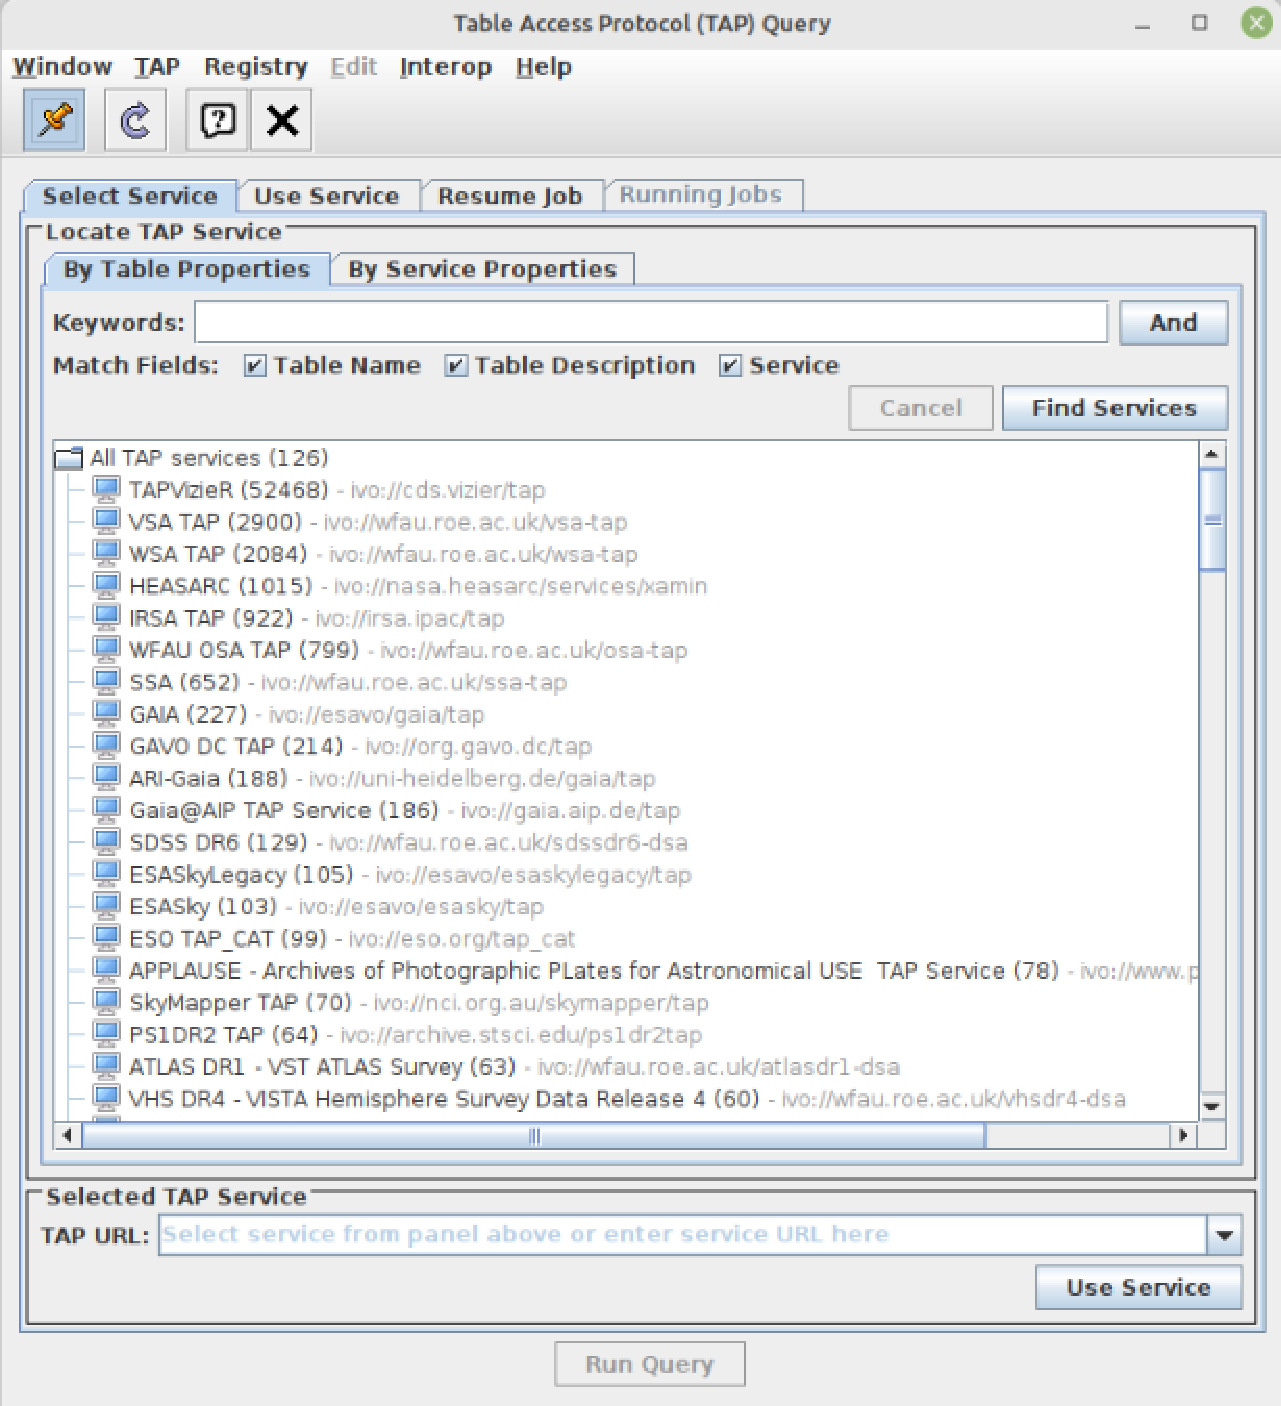
\includegraphics[width=0.7\textwidth]{img/tesis/tap_query.pdf}
	\caption{PDF}
	\label{fig:tap_query}
\end{figure}


\begin{figure}
	\centering
	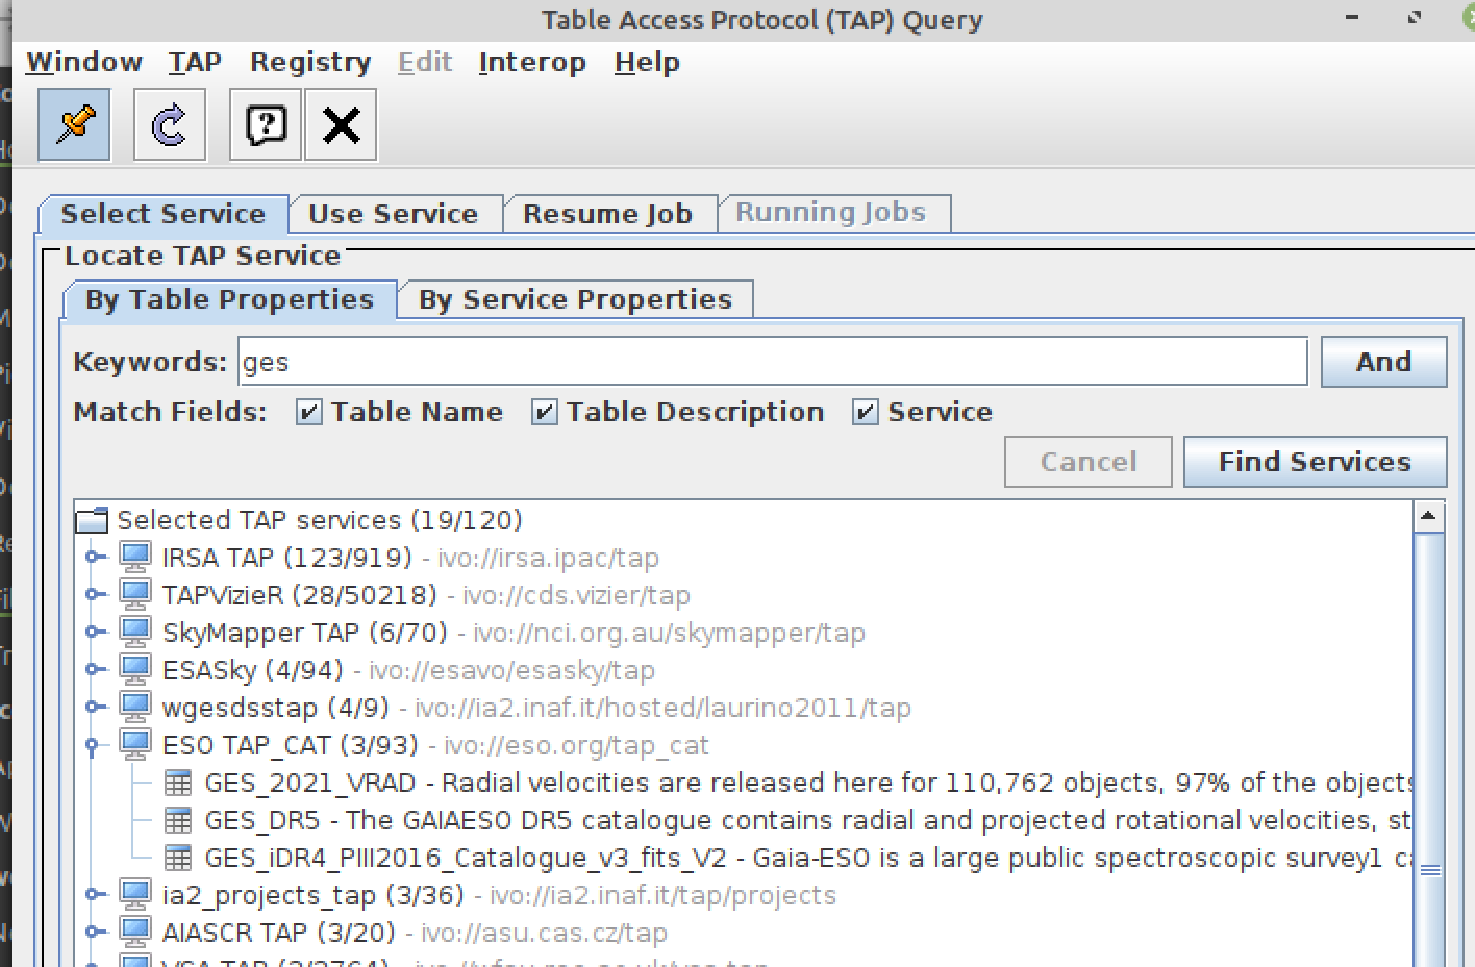
\includegraphics[width=0.7\textwidth]{img/tesis/tap_ges_service.pdf}
	\caption{PDF}
	\label{fig:tap_ges_service}
\end{figure}

\begin{figure}
	\centering
	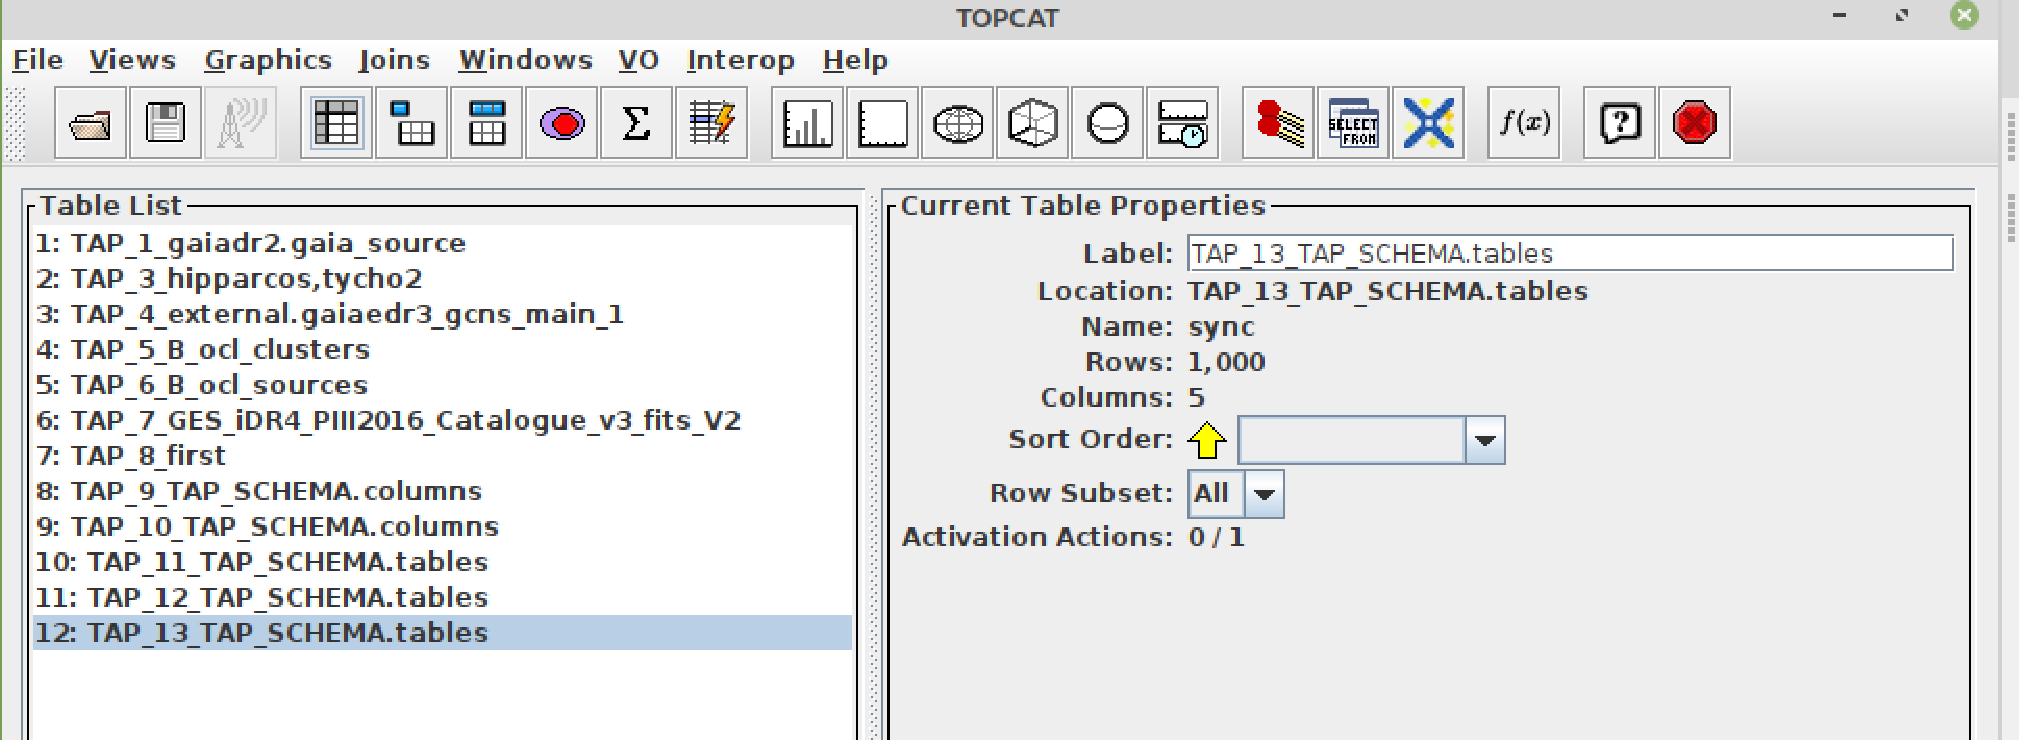
\includegraphics[width=0.7\textwidth]{img/tesis/tap_multi_sources.pdf}
	\caption{PDF}
	\label{fig:tap_multi_services}
\end{figure}

\begin{figure}
	\centering
	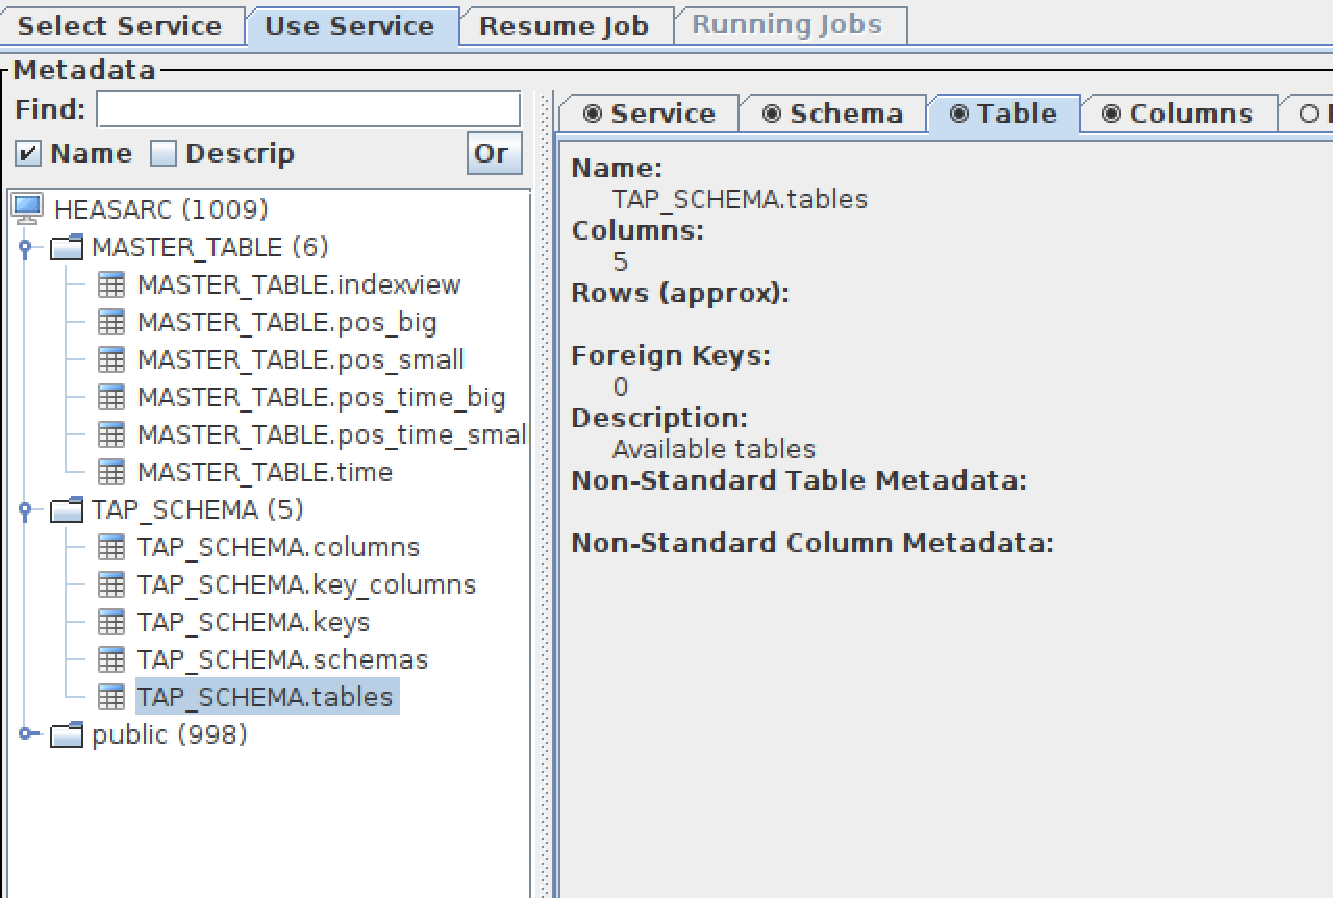
\includegraphics[width=0.7\textwidth]{img/tesis/tap_schema.pdf}
	\caption{PDF}
	\label{fig:tap_schema}
\end{figure}

\begin{figure}
	\centering
	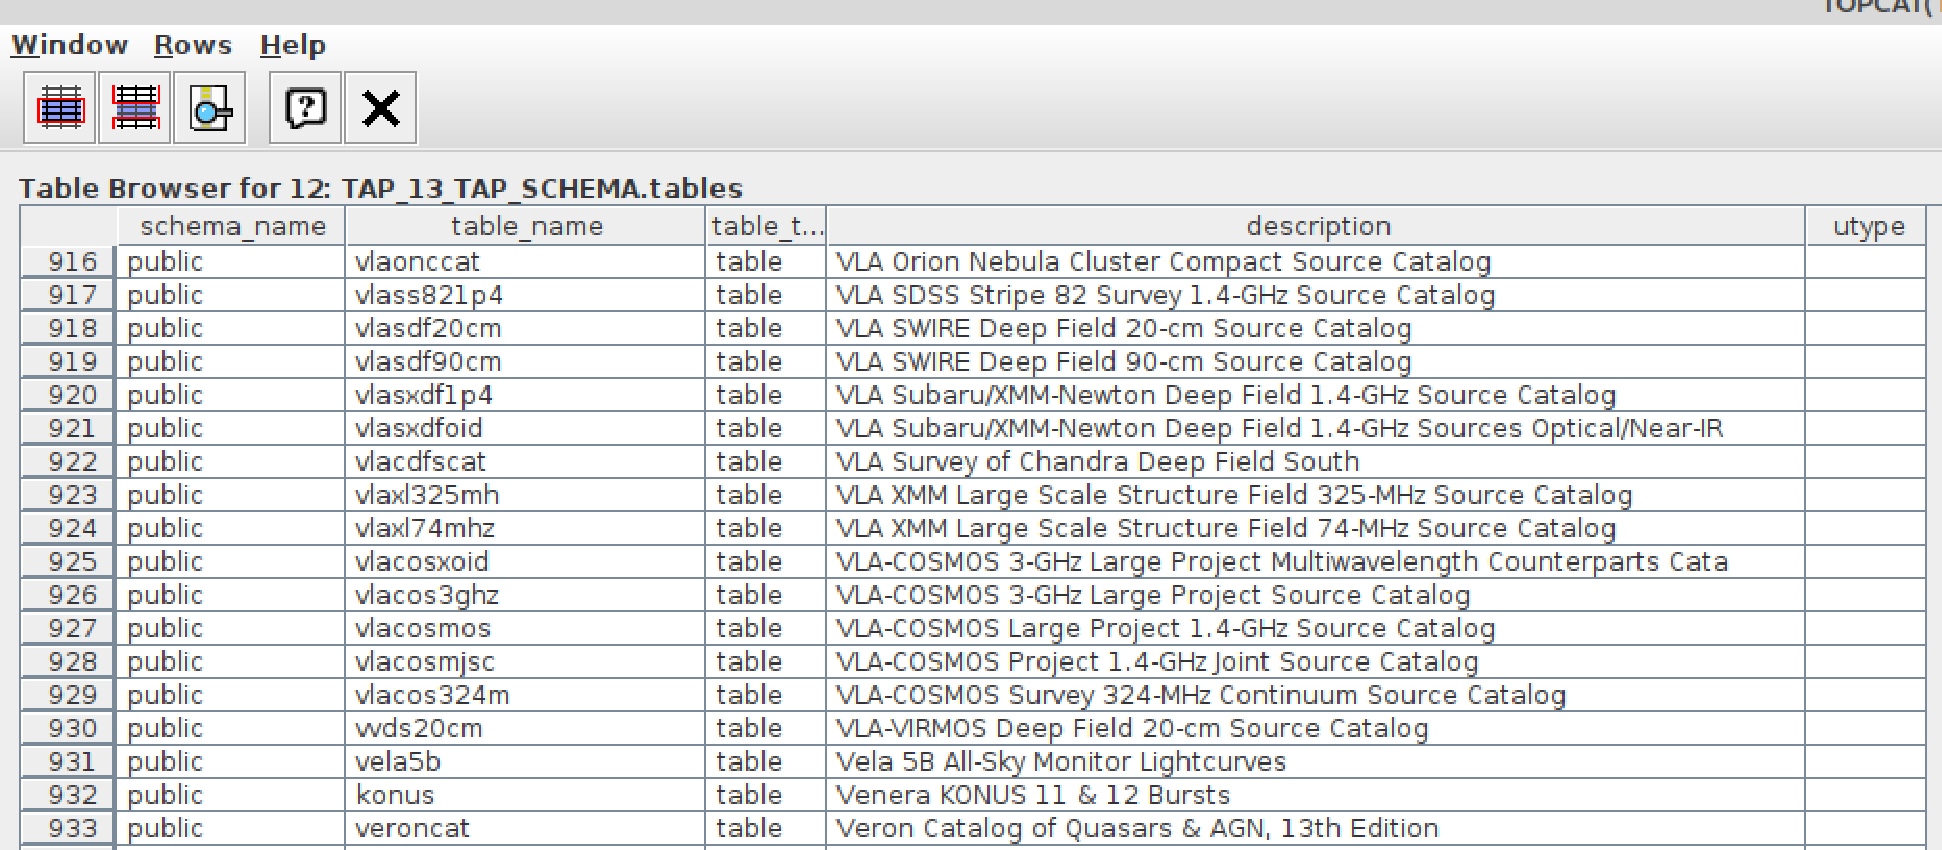
\includegraphics[width=0.7\textwidth]{img/tesis/tap_schema_detail.pdf}
	\caption{PDF}
	\label{fig:tap_schema_detail}
\end{figure}

\begin{figure}
	\centering
	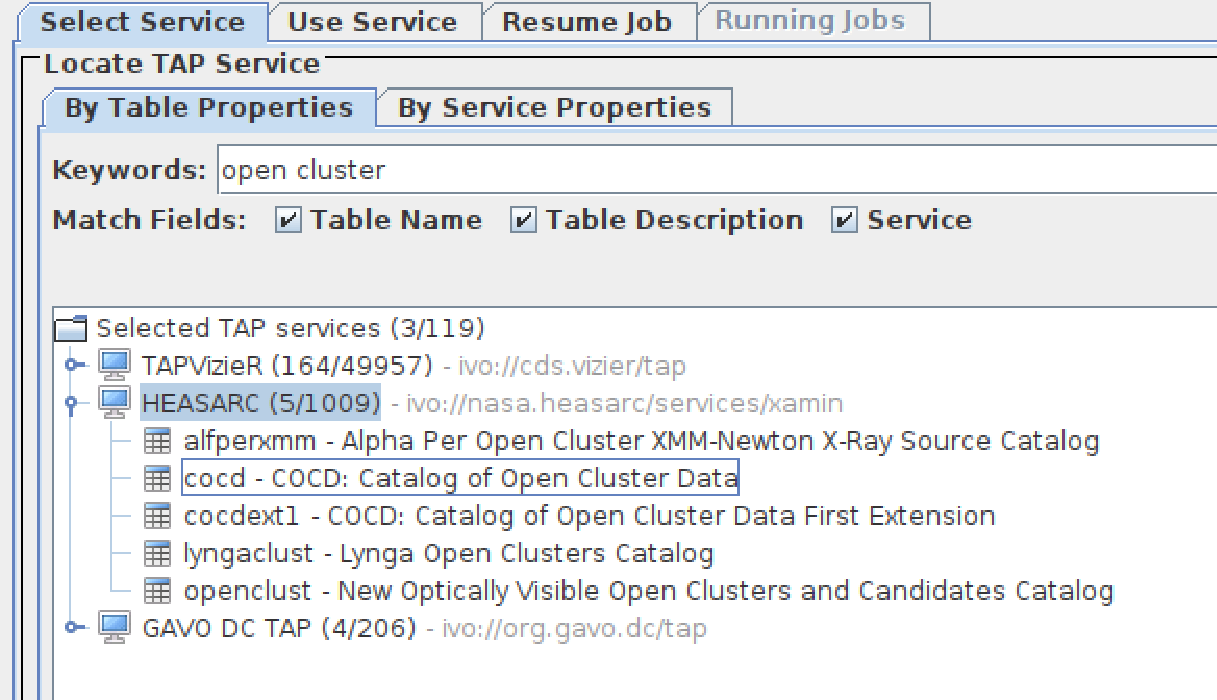
\includegraphics[width=0.7\textwidth]{img/tesis/tap_service.pdf}
	\caption{PDF}
	\label{fig:tap_service}
\end{figure}






\section{Catálogos de datos}
Una etapa fundamental de toda investigación es la de la confrontación de los datos arrojados con los modelos contra los disponibles en la literatura ya existente,

\subsection{Gaia}
El catálogo Gaia es un mapa tridimensional completo de la Vía Láctea, creado utilizando datos del telescopio espacial Gaia. Éste contiene datos de alrededor de 1.46 mil millones de estrellas, entre los que se encuentra sus posiciones en el cielo, paralaje y movimiento propio. Además, incluye sus magnitudes en diferentes bandas espectrales para una gran cantidad de ellas. El catálogo Gaia es particularmente útil para estudiar estrellas similares al Sol, ya que proporciona un censo único de estrellas dentro de 100 pc de nuestro Sol. Esto lo convierte en un recurso invaluable para los astrónomos y astrofísicos que buscan comprender mejor las propiedades y la evolución de estas estrellas.\par

\subsection{Gaia-ESO Spectroscopic Survey (GES)}
GES es un catálogo público enfocado al análisis espectroscópico de un número importante de estrellas recogidas en el catálogo Gaia. Se llevó a cabo con el instrumento FLAMES en el VLT. Su objetivo es proporcionar una visión homogénea de las distribuciones de cinemática y abundancias elementales en la Vía Láctea. Dentro de la iniciativa GES se han observado más de 100 000 estrellas, proporcionando velocidades radiales y rotacionales proyectadas, parámetros estelares tales como: temperatura efectiva, gravedad superficial y metalicidad, abundancias de varios elementos, entre los que se encuentra el Litio, y parámetros específicos para rastrear la acreción y actividad en estrellas jóvenes. El catálog GES es único en lo que se refiere a la observación de estrellas de todos los tipos espectrales con análisis dedicados y especializados, lo que la hace particularmente útil para estudiar estrellas similares al Sol.\par

\subsection{Combinando Gaia y GES}

La combinación de los datos de los catálogos Gaia y GES puede proporcionar una visión completa de las propiedades y evolución de las estrellas similares al Sol. El catálogo Gaia proporciona datos de posición precisos y paralajes, mientras que la GES ofrece información espectroscópica detallada. Esta combinación permite una comprensión más completa de estas estrellas, incluyendo su cinemática, composiciones químicas y potencial para albergar planetas. Al proporcionar una visión más completa y detallada de estas estrellas, podemos obtener una comprensión más profunda de las propiedades y evolución de las estrellas similares al Sol, lo que representa una fuente de información que se antoja invaluable para la investigación en astrofísica. Estamos ante un conjunto de herramientas poderoso para cualquier astrofísico que estudie estrellas similares al Sol.\par

En el caso de las abundancias de Litio, y como ya hemos apuntado, éste es un elemento clave en el estudio de la astrofísica estelar, ya que su abundancia puede proporcionar información valiosa sobre la edad y la historia de las estrellas. Sin embargo, la determinación precisa de las abundancias de Litio puede ser un desafío debido a la complejidad de las líneas espectrales del Litio. GES nos asiste en nuestra investigación aportando su análisis especializado y dedicado de estrellas de todos los tipos espectrales, convirtiéndose así en una herramienta fundamental a la hora de afrontar este desafío.\par

Por otra parte, tenemos información precisa sobre la velocidad angular de las estrellas. Gaia es capaz de medir la velocidad angular de las estrellas con una precisión sin precedentes, y ésta nos aporta información es crucial para estudiar y entender la rotación de las estrellas, su evolución y estructura interna. Combinado esta información con las abundancia de Litio podemos establecer hipótesis y validar las mismas acerca del impacto de la velocidad angular sobre el Litio. Paralelamente, la velocidad angular juega un papel crucial en el análisis de la presencia e intensidad de un campo magnético en las estrellas. Los campos magnéticos son responsables de la pérdida de momento angular en las estrellas jóvenes y son la principal fuente de energía detrás de una amplia gama de fenómenos dinámicos (llamaradas, emisión de rayos X, manchas estelares) que ocurren en las capas superficiales del Sol y otras estrellas. Por lo tanto, la medición precisa de la velocidad angular de una estrella puede proporcionar información valiosa sobre la presencia e intensidad de su campo magnético.\par

Otra fuente de información valiosa para nuestra investigación procedente de ambos catálogos es la referida a los cúmulos abiertos. Los cúmulos abiertos son grupos de estrellas que se formaron a partir de la misma nube de gas y polvo. Por lo tanto, todas las estrellas de un cúmulo abierto tienen aproximadamente la misma edad y composición química inicial. Esto los convierte en laboratorios naturales para estudiar la evolución de las estrellas a través de sus diferentes etapas. Gaia ha observado una gran cantidad de cúmulos abiertos, proporcionando datos detallados sobre sus miembros. En paralelo, GES también ha observado un gran número de ellos en un rango amplio de edades. La combinación de ambas fuentes permite estudiar la estructura y dinámica de este tipo de cúmulos, y usarlos para restringir y mejorar los modelos de evolución estelar, algo que hemos puesto en práctica en nuestra investigación.\par

Como acabamos de adelantar, la investigación de los campos magnéticos en estrellas similares al Sol. y en particular de aquéllas que se encuentran en cúmulos abiertos, se beneficia enormemente de los datos proporcionados por ambos catálogos. Los campos magnéticos juegan un papel importante en todas las etapas de la evolución estelar. En estrellas similares al Sol, se generan en las capas convectivas exteriores. Estudiar los campos magnéticos a gran escala de estas estrellas puede mejorar nuestra comprensión sobre los mismos y proporcionar restricciones observacionales para los modelos que estudian cómo se generan, la topología que presentan y sus intensidades. Los datos de los catálogos nos asisten a la hora de identificar y estudiar las estrellas con alta actividad magnética, lo que puede proporcionar pistas sobre la dinámica interna de las estrellas y su evolución. Combinando esta información con la velocidad angular, nos puede proporcionar con indicios de cómo se interrelacionan ambos fenómenos. Adicionalmente, cruzando estos datos con la información de los cúmulos abiertos, obtenemos una visión más clara de cómo los campos magnéticos varían entre las estrellas de la misma edad y composición química.\par

\begin{figure}
	\centering
	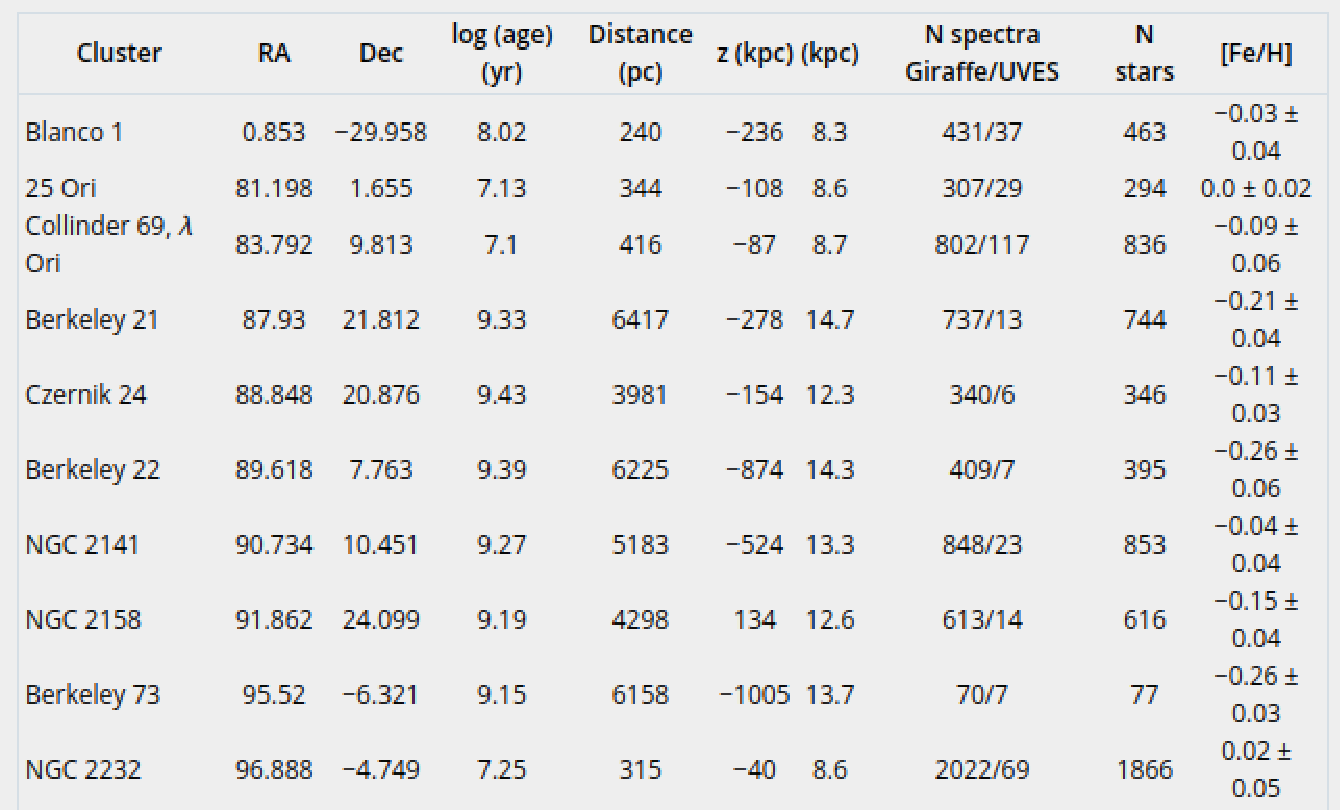
\includegraphics[width=0.7\textwidth]{img/tesis/open_cluster_sample.pdf}
	\caption{Tabla obtenida de \cite{Bragaglia2022}. Las columnas 1 a 7 listan la denominación del cúmulo, las coordenadas de ascensión recta y declinación, la edad estimada del cúmulo, la distancia en parsecs (módulo de distancia convertido), la posición Z en coordenadas cartesianas galácticas, y la distancia desde el centro galáctico suponiendo que el Sol está a 8340pc. Las columnas 8 y 9 enumeran el número de espectros y objetivos, mientras que la media de [Fe/H] y la desviación estándar se dan en la columna 10.}
	\label{fig:open_cluster_sample}
\end{figure}




La abundancia de Litio puede proporcionar información valiosa sobre la edad y la historia de las estrellas. En particular, puede ayudar a rastrear la mezcla convectiva en el interior de las estrellas, que está influenciada por la rotación estelar. La rotación, a su vez, puede ser modulada por la presencia de campos magnéticos a través del frenado magnético.

Además, en estrellas jóvenes y de baja masa, la presencia de fuertes campos magnéticos puede inhibir la convección, alterando el transporte de energía desde el interior de la estrella. Esto puede afectar la tasa de quema de Litio, lo que resulta en una mayor abundancia de Litio en la superficie de la estrella de lo que se esperaría de lo contrario.

Por lo tanto, al estudiar las abundancias de Litio en las estrellas, los astrónomos pueden obtener pistas sobre la intensidad de los campos magnéticos en el interior de las estrellas. Sin embargo, la interpretación de las abundancias de

Los campos magnéticos en las estrellas pueden tener un impacto significativo en la abundancia de Litio presente en ellas. El Litio se quema fácilmente a una temperatura relativamente baja (2.5 x $10^6$ K) en el interior estelar³. Por lo tanto, es un diagnóstico extraordinariamente sensible de la estructura y evolución estelar³.

La abundancia de Litio puede proporcionar información valiosa sobre la edad y la historia de las estrellas. En particular, puede ayudar a rastrear la mezcla convectiva en el interior de las estrellas, que está influenciada por la rotación estelar. La rotación, a su vez, puede ser modulada por la presencia de campos magnéticos a través del frenado magnético.

Además, en estrellas jóvenes y de baja masa, la presencia de fuertes campos magnéticos puede inhibir la convección, alterando el transporte de energía desde el interior de la estrella. Esto puede afectar la tasa de quema de Litio, lo que resulta en una mayor abundancia de Litio en la superficie de la estrella de lo que se esperaría de lo contrario¹.

Por lo tanto, al estudiar las abundancias de Litio en las estrellas, los astrónomos pueden obtener pistas sobre la intensidad de los campos magnéticos en el interior de las estrellas. Sin embargo, la interpretación de las abundancias de Litio puede ser compleja, ya que también pueden ser influenciadas por otros factores, como la metalicidad de la estrella y la eficiencia de la convección¹.

En resumen, aunque el Litio no proporciona una medida directa de los campos magnéticos estelares, su abundancia en las estrellas puede ofrecer valiosas pistas sobre la actividad magnética en el interior estelar. Esto hace que las mediciones de las abundancias de Litio, como las proporcionadas por la Encuesta Espectroscópica Gaia-ESO (GES), sean una herramienta importante para la investigación de los campos magnéticos en las estrellas.

Source: Conversation with Bing, 1/25/2024
(1) [2006.01899] Study of the effects of magnetic braking on the lithium .... https://arxiv.org/abs/2006.01899.
(2) Study of the effects of magnetic braking on the lithium abundances of .... https://academic.oup.com/mnras/article/496/2/1343/5851759.
(3) Enhanced lithium depletion in Sun-like stars with orbiting planets - Nature. https://www.nature.com/articles/nature08483.pdf.
(4) undefined. https://doi.org/10.1093/mnras/staa1569.

Source: Conversation with Bing, 1/25/2024
(1) Effect of magnetic fields on Lithium depletion of solar-type stars. https://www.cambridge.org/core/services/aop-cambridge-core/content/view/054CD22CB5342846A1EC5552F7DED8FE/S1743921313002512a.pdf/effect-of-magnetic-fields-on-lithium-depletion-of-solar-type-stars.pdf.




En resumen, cada uno de estos enfoques ofrece una perspectiva única y valiosa sobre la naturaleza y la evolución de estrellas. La combinación de los catálogos Gaia y GES proporciona una visión completa y detallada de las estrellas similares al Sol. La información sobre las abundancias de Litio, la velocidad angular y los datos de los cúmulos abiertos, en particular, puede arrojar luz sobre la cinemática, la composición química, la edad y la historia de estas estrellas, así como ser una herramienta muy potente para ofrecer una perspectiva única y valiosa sobre la naturaleza y la evolución de los campos magnéticos estelares.  En resumen, una fuente de datos invaluable para cualquier astrofísico que estudie estrellas similares al Sol.\par





Source: Conversation with Bing, 1/25/2024
The Gaia-ESO Survey: Calibrating the lithium–age relation with open .... https://arxiv.org/pdf/2009.00610.pdf.
Interferometric Observations of Magnetic Fields in Forming Stars. https://www.frontiersin.org/articles/10.3389/fspas.2019.00003/full.
ESO Survey: 3D dynamics of young groups and clusters from GES and Gaia .... https://arxiv.org/pdf/2311.08358.pdf.
Stellar magnetic fields and surface structures - Uppsala University. https://www.physics.uu.se/research/astronomy-and-space-physics/research/stars/magnetism/.
The Role of Magnetic Fields in Protostellar Outflows and Star Formation. https://www.frontiersin.org/articles/10.3389/fspas.2019.00054/full.
The Gaia-ESO Survey: Membership probabilities for stars in 32 open .... https://arxiv.org/pdf/2006.09423v1.pdf.
undefined. https://doi.org/10.3389/fspas.2019.00054.
Source: Conversation with Bing, 1/25/2024
[1310.5562] Magnetic fields of Sun-like stars - arXiv.org. https://arxiv.org/abs/1310.5562.
undefined. https://doi.org/10.1017/S1743921314002026.
Membership of stars in open clusters using random forest with gaia data .... https://link.springer.com/article/10.1140/epjs/s11734-021-00205-x.
Evidence of New Magnetic Transitions in Sun-like Stars from Gaia Data. https://www.spacedaily.com/reports/Evidence of New Magnetic Transitions in Sun like Stars from Gaia Data 999.html.
undefined. https://doi.org/10.48550/arXiv.1310.5562.



\endinput
%--------------------------------------------------------------------
% FIN DEL CAPÍTULO. 
%--------------------------------------------------------------------